\documentclass[12pt]{article}
\usepackage[italian]{babel}
\usepackage{graphicx}
\usepackage[section]{placeins}
\usepackage{amsmath}% http://ctan.org/pkg/amsmath
\usepackage{enumitem}
\usepackage{graphicx}
\usepackage{hyperref}
\usepackage[section]{placeins}

\title{Metodi Informatici per la Gestione Aziendale - Relazione Finale Progetto}
\author{Giuseppe Facchi}
\date{A.A. 2020-2021}

\begin{document}
\maketitle
\newpage
\tableofcontents
\newpage

\section{Panoramica}
Lo scopo principale dell'applicazione vertono sulla predizione e sulla classificazione della qualità di varianti del vino bianco Portoghese \textit{vinho verde} in base alle loro proprietà chimiche. Dopo l'ottenimento di accettabili modelli di \textbf{regressione} e di \textbf{classificazione}, sarà possibile effettuare analisi di mercato per poter produrre varianti di vino sempre più perfezionate e progettare marketing strategies basate sul target di utenza da soddisfare.
\paragraph{Vinho Verde} è una denominazione che annovera tipologie non solo di vino bianco, ma anche di vino rosso e rosato. Viene prodotto in tutto il Portogallo da monovitigni o in uvaggio, è leggermente frizzante e presenta aromi di miele, di frutta e di fiori di campo.
\begin{figure}[!htb]
    \centering
    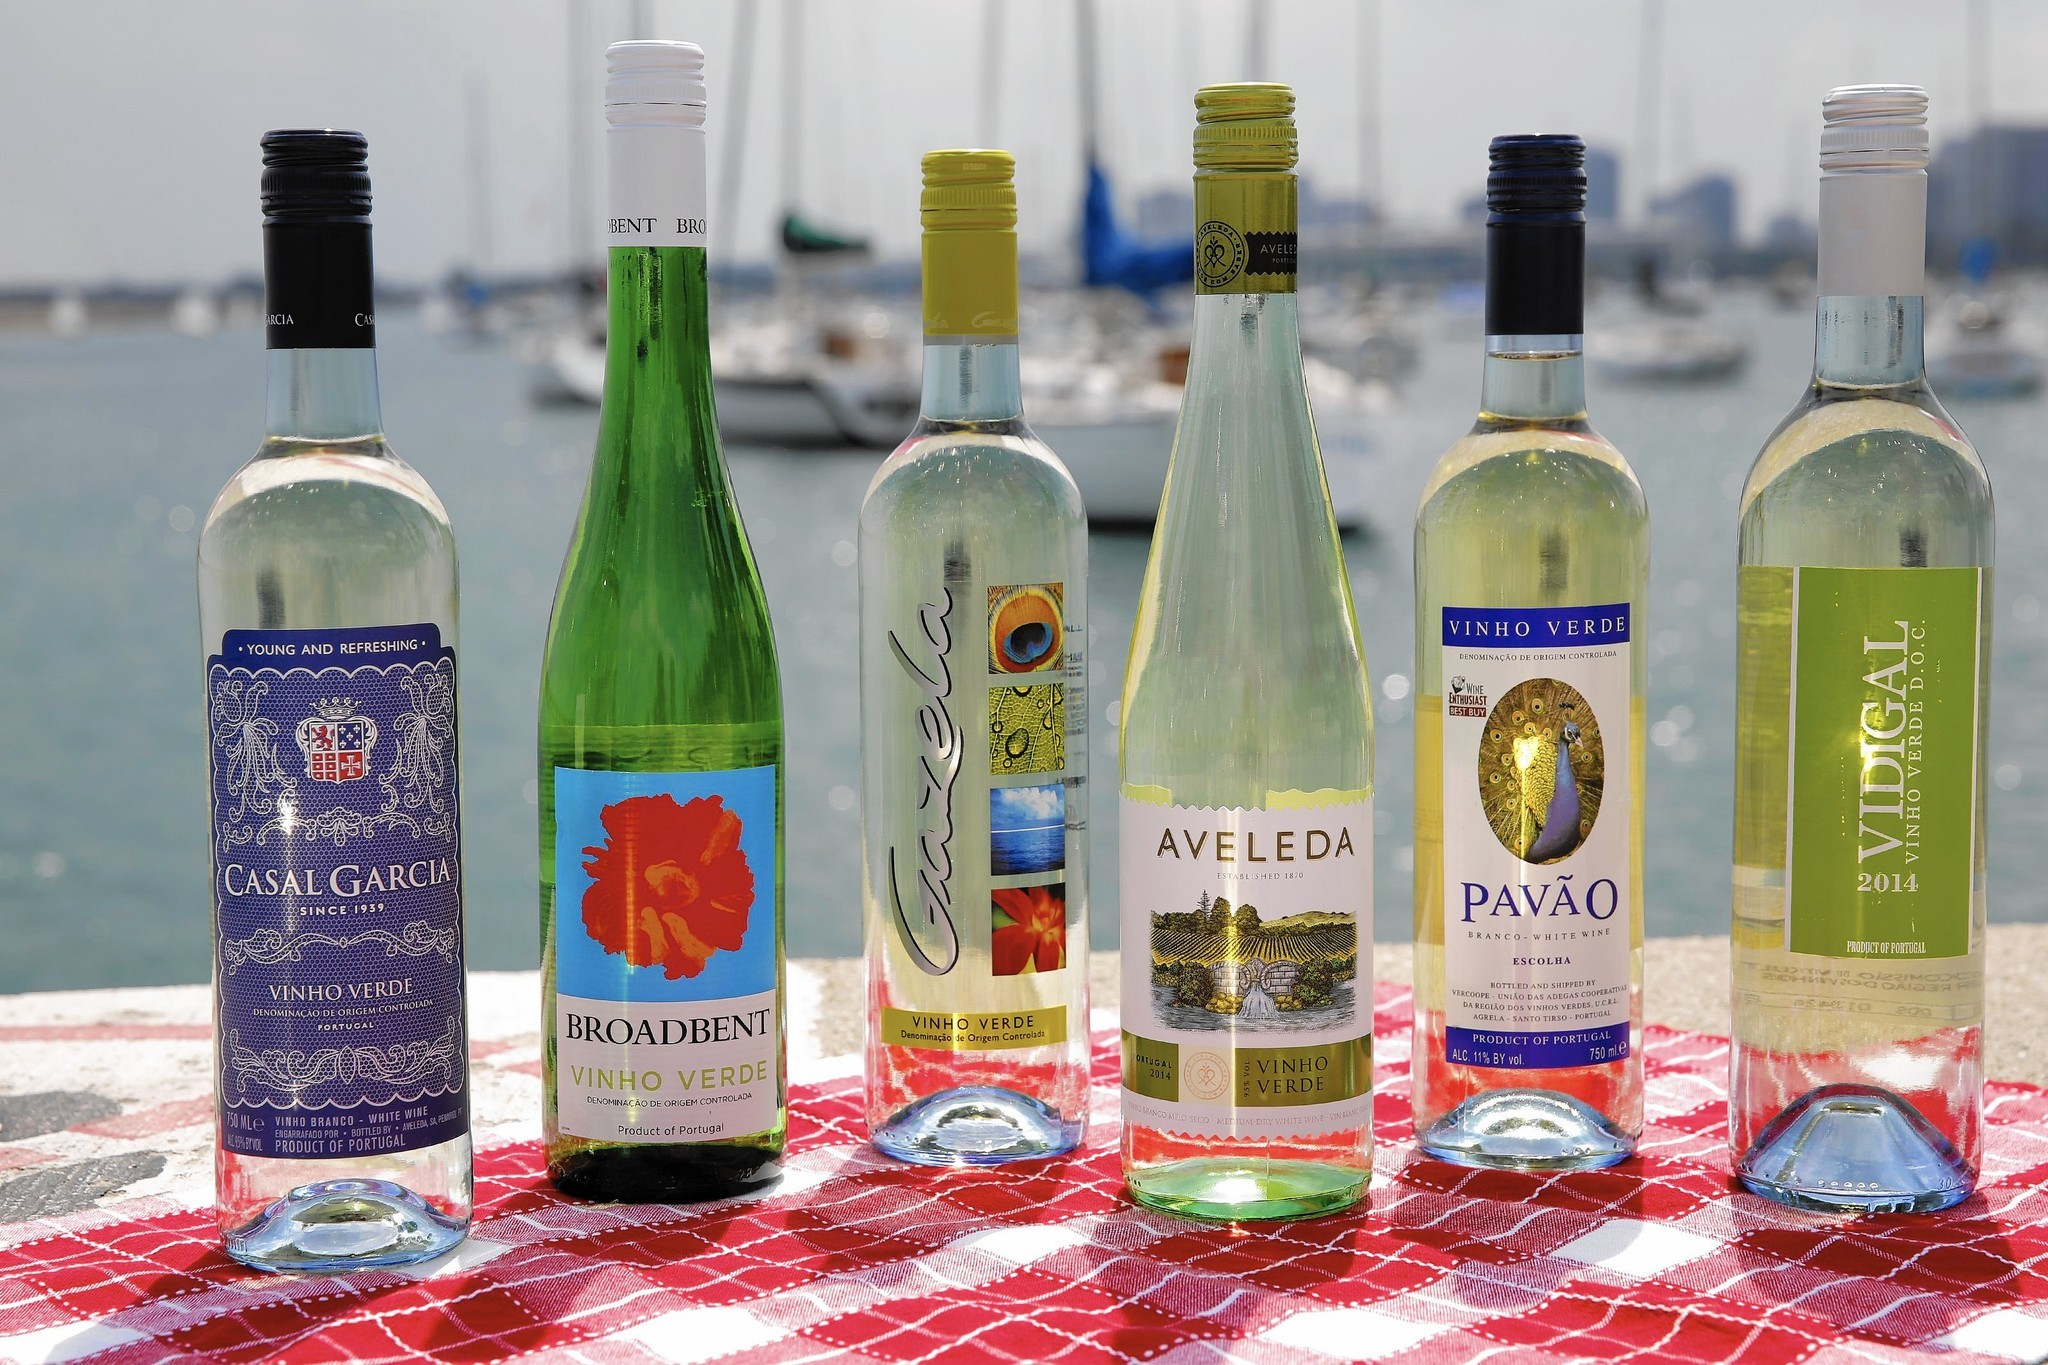
\includegraphics[width=1\textwidth]{immagini/vin.jpg}
    \caption{Varianti di Vinho Verde portoghese}
\end{figure}
\FloatBarrier
\newpage
\section{Data Acquisiton}
\subsection{Descrizione del dataset}
Il dataset utilizzato è reperibile a questo \href{https://archive.ics.uci.edu/ml/datasets/Wine+Quality}{link}. Tra le due collezioni è stata esaminata quella relativa alle varianti di vinho verde bianco.
Di seguito le sue principali caratteristiche:
\begin{itemize}
    \item N° totale di osservazioni: \textbf{4898}
    \item N° di variabili: \textbf{12}
\end{itemize}
Ogni variante di vinho verde è descritta tramite valori di
\begin{itemize}
    \item \textbf{Acidi Non Volatili}: Gli acidi non volatili sono composti chimici che non possono essere rapidamente vaporizzati. Ciò è principalmente dovuto al fatto che la pressione di vapore dell'acido a temperatura ambiente normale non è sufficientemente elevata da vaporizzare facilmente
    \item \textbf{Acidi Volatili}: Gli acidi volatili sono composti chimici che subiscono rapidamente la vaporizzazione. Questa rapida vaporizzazione è il risultato di una pressione di vapore elevata a temperatura ambiente normale. Pertanto, gli acidi volatili possono subire vaporizzazione senza riscaldamento o qualsiasi altra forza esterna
    \item \textbf{Acido Citrico}: Viene utilizzato nel vino per prevenire le ossidazioni e si presenta, come additivo o acidificante, sotto forma di polverina bianca e cristallina pura
    \item \textbf{Zuccheri Residui}: Determinano la maggiore o minore dolcezza del vino
    \item \textbf{Cloruri}: Determinano la sensazione di sapidità
    \item \textbf{Anidride Solforosa Libera}: Forme liberabili in seguito ad acidificazione
    \item \textbf{Anidride Solforosa Totale}: Usata in giuste quantità migliora la qualità e prolunga la durata del vino
    \item \textbf{Densità}
    \item \textbf{PH}: Indica l'acidità/basicità) del vino
    \item \textbf{Solfiti}: Funzione principale di conservanti, per contrastare l’ossidazione dei cibi e prevenire lo sviluppo microbico indesiderato
    \item \textbf{\% Alcol}: Numero di parti in volume di alcol etilico, alla temperatura di 20 °C, contenuta in 100 parti in volume del prodotto considerato alla stessa temperatura
    \item \textbf{Qualità}: Valutazione soggettiva del vino da 1 a 10
\end{itemize}
\subsection{Descrizione dei valori delle variabili}
Come evidenziato dalla seguente infografica non sono presenti missing values nel dataset in analisi. Sarà quindi possibile proseguire l'analisi senza effettuare operazioni di modifica dell'integrità del dataset.
\begin{figure}[!htb]
    \centering
    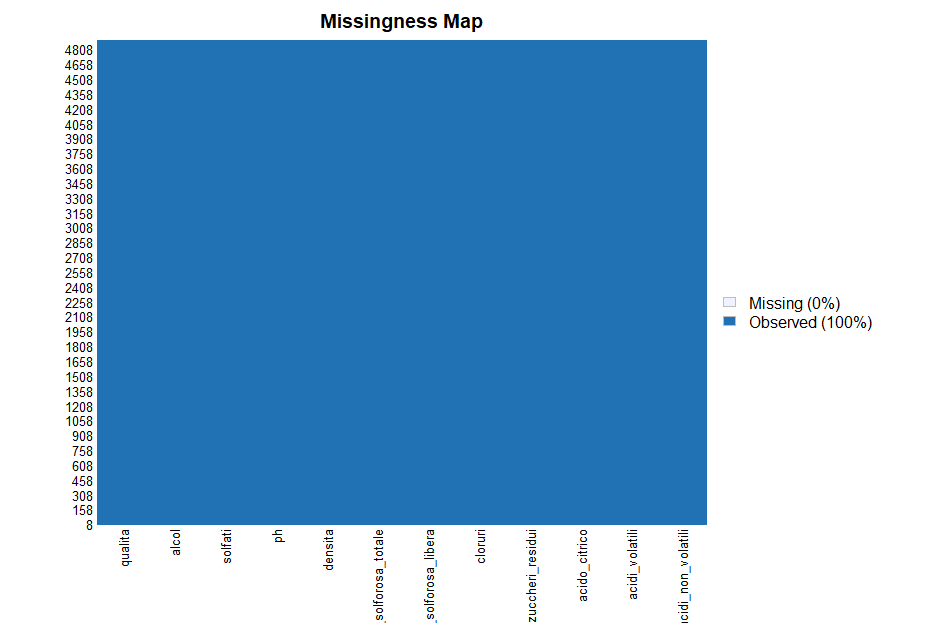
\includegraphics[width=1\textwidth]{immagini/missmap.png}
    \caption{Missmap del dataset in analisi}
\end{figure}
\FloatBarrier
Una panoramica generale dei valori del dataset è illustrata di seguito. Tutte le variabili sono rappresentate da dati numerici:
\begin{figure}[!htb]
    \centering
    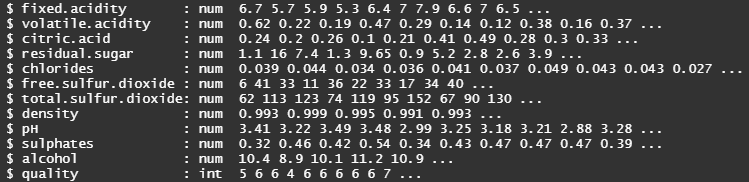
\includegraphics[width=1\textwidth]{immagini/str.png}
    \caption{Panoramica tipi di variabile}
\end{figure}
\FloatBarrier
Essendo le variabili di tipo numerico è possibile estrarre numerose statistiche riguardo la loro distribuzione tra cui minimi, massimi, somma, mediana, media, varianza e deviazione standard. Di seguito un sommario del loro calcolo:
\begin{figure}[!htb]
    \centering
    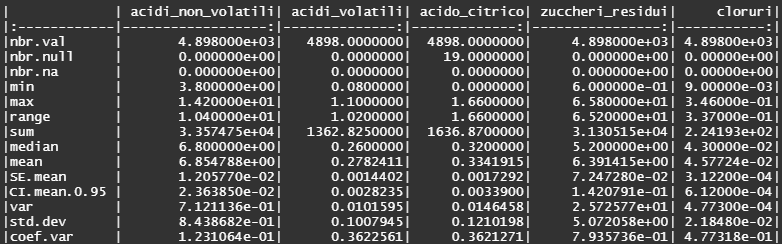
\includegraphics[width=0.8\textwidth]{immagini/sum.png}
\end{figure}
\begin{figure}[!htb]
    \centering
    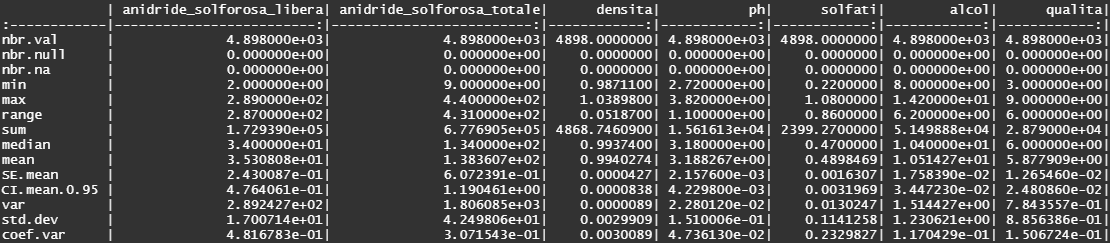
\includegraphics[width=1\textwidth]{immagini/sum1.png}
    \caption{Calcolo delle principali statistiche riguardo la distribuzione dei valori delle variabili}
\end{figure}
\FloatBarrier
Da una prima analisi delle statistiche è possibile notare come la qualità presenti una media di 5.87, molto vicino alla mediana di 6 facendo notare come la distribuzione dei vini sia centrata molto su una qualità di valore 6. Varianza e deviazione standard delle variabili risultano molto contenute, rispecchiando una minima dispersione dei valori.
\newpage
\subsection{Descrizione delle distribuzioni delle variabili}
Per effettuare un'analisi approfondita delle variabili è possibile rappresentarne le distribuzioni attraverso istogrammi di occorrenza, box plots, q-q plots e densità.
\subsubsection{Qualità}
\begin{figure}[!htb]
    \centering
    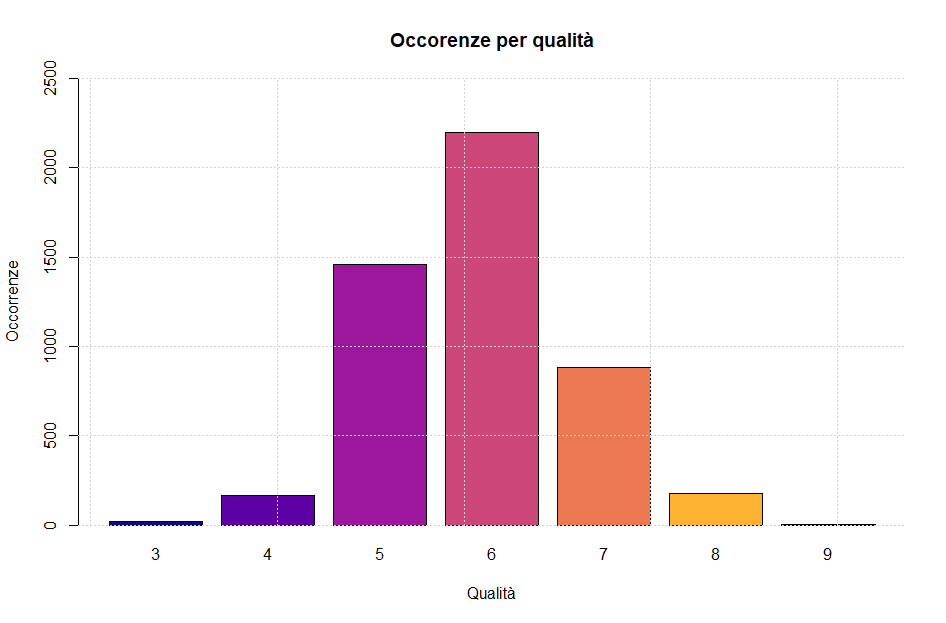
\includegraphics[width=1\textwidth]{immagini/qua.png}
    \caption{Istogramma delle occorrenze di vini rispetto alla loro qualità}
\end{figure}
\FloatBarrier
Come si denota dall'istogramma delle occorrenze dei vini in base alla loro qualità, la presenza di vini di qualità 6 è predominante, mentre la loro distribuzione per valori minori e maggiori di 6 è pressoché equivalente, questo consentirà successivamente la creazione di una feature aggiuntiva riguardo il gusto del vino: utilizzando la qualità 6 per denotare un gusto normale, una qualità maggiore di 6 per denotare un buon gusto e una qualità minore di 6 per denotare un cattivo gusto.
\newpage
\subsubsection{Acidi non volatili}
\begin{figure}[!htb]
    \centering
    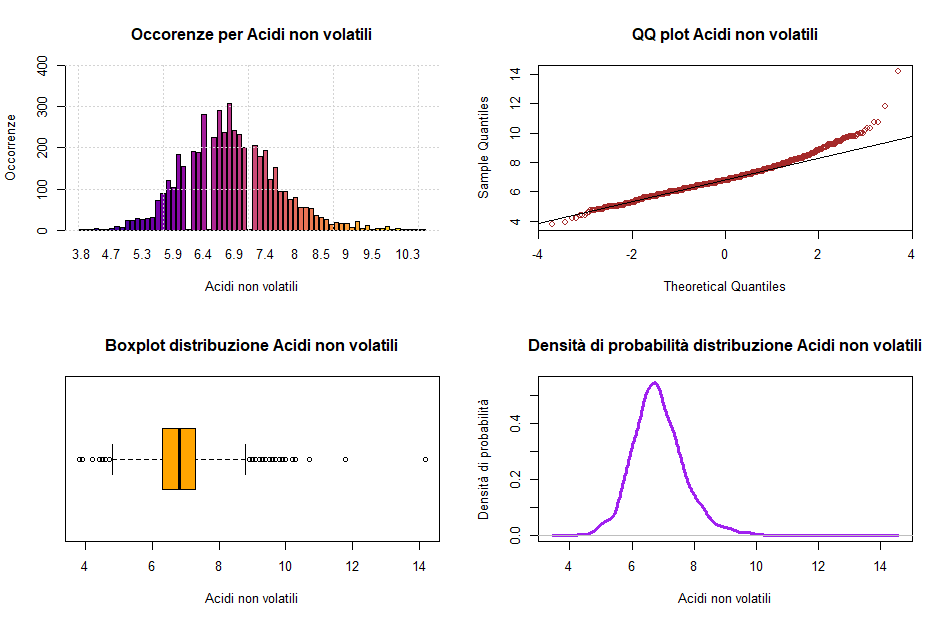
\includegraphics[width=1\textwidth]{immagini/acnon.png}
    \caption{Plots per la descrizione della distribuzione della variabile di Acidi non volatili}
\end{figure}
\FloatBarrier
Dall'insieme dei grafici relativi alla distribuzione degli acidi non volatili è possibile concludere che la maggior parte dei valori seguano una distribuzione normale, con l'eccezione di numerosi outliers visualizzabili nel boxplot nel range dal terzo all'ultimo quartile.
\newpage
\subsubsection{Acidi volatili}
\begin{figure}[!htb]
    \centering
    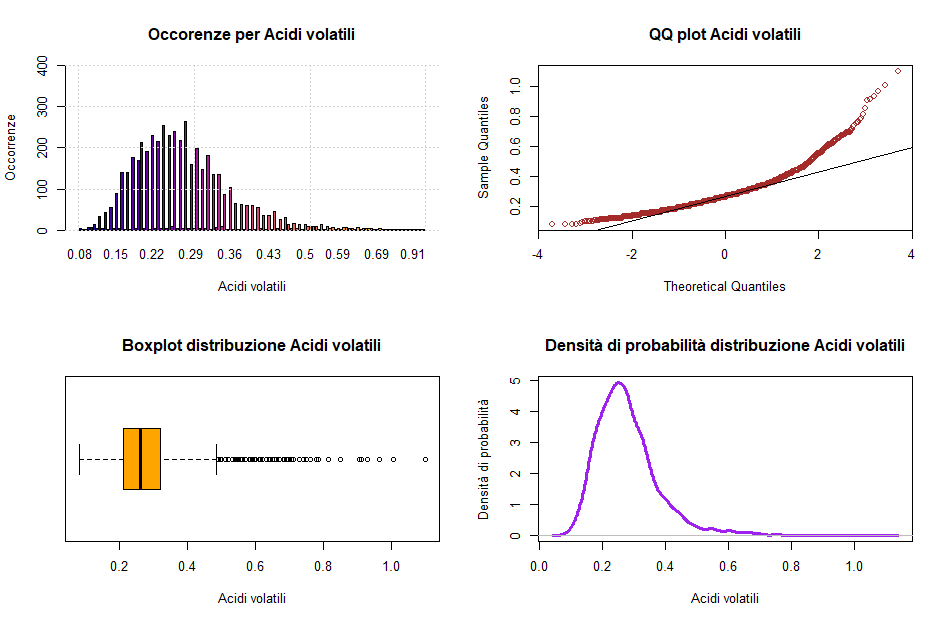
\includegraphics[width=1\textwidth]{immagini/acvol.png}
    \caption{Plots per la descrizione della distribuzione della variabile di Acidi volatili}
\end{figure}
\FloatBarrier
A differenza degli acidi non volatili, dall'insieme dei grafici relativi alla distribuzione degli acidi volatili è possibile concludere che i valori si discostano maggiormente da una distribuzione normale. Infatti anche dal boxplot è possibile notare una grossa presenza di outliers per alti valori di acidi volatili.
\newpage
\subsubsection{Acido citrico}
\begin{figure}[!htb]
    \centering
    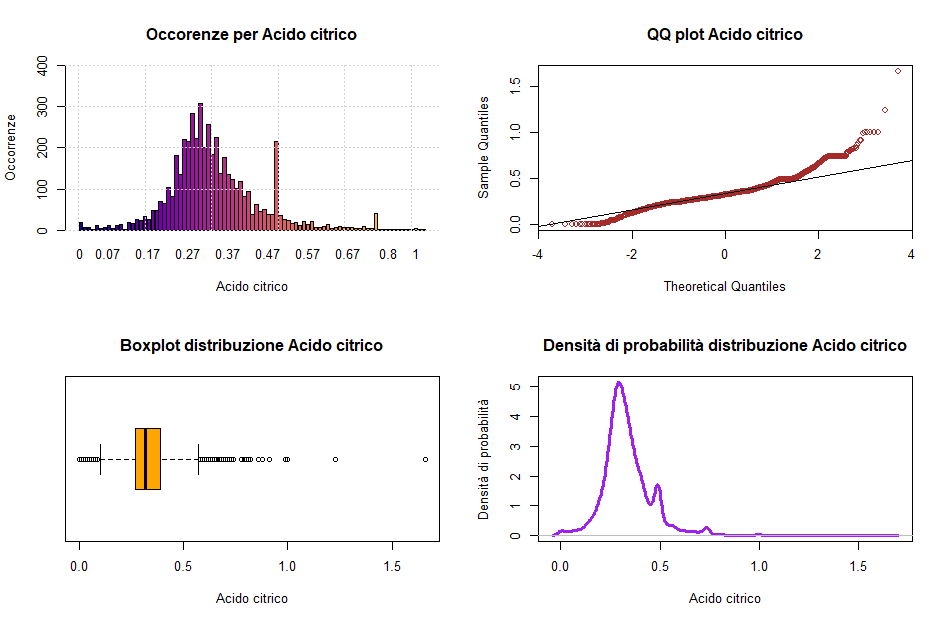
\includegraphics[width=1\textwidth]{immagini/accit.png}
    \caption{Plots per la descrizione della distribuzione della variabile di Acido citrico}
\end{figure}
\FloatBarrier
L'insieme dei grafici relativi alla distribuzione dei valori di acido citrico ne denota una certa irregolarità. Questa considerazione può essere fatta dall'osservazione di numerosi outliers, sia per bassi che alti valori, della distribuzione dei valori di acido citrico. Spicca un valore su tutti in corrispondenza di 2 g/L.
\newpage
\subsubsection{Zuccheri residui}
\begin{figure}[!htb]
    \centering
    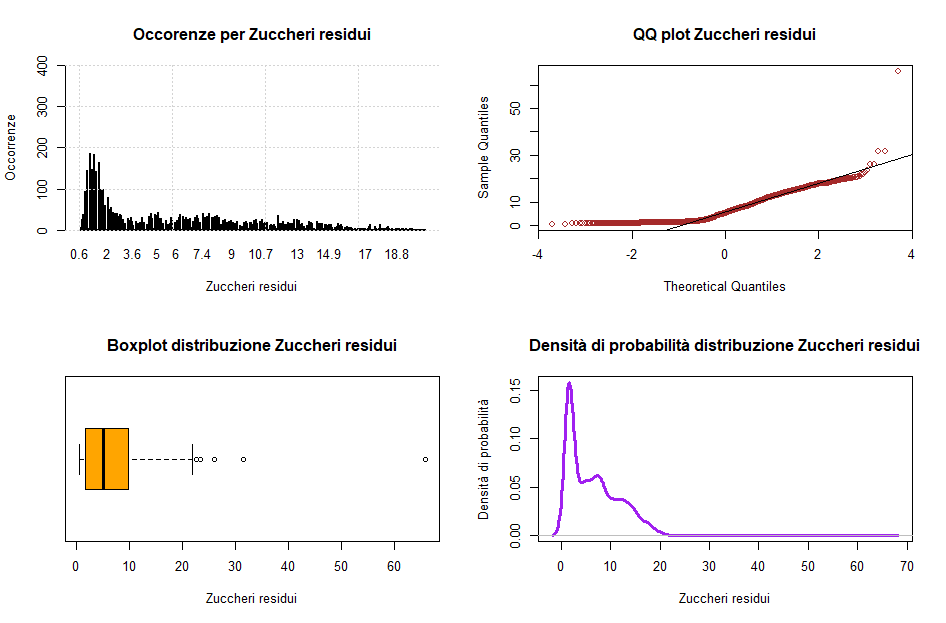
\includegraphics[width=1\textwidth]{immagini/zr.png}
    \caption{Plots per la descrizione della distribuzione della variabile di Zuccheri residui}
\end{figure}
\FloatBarrier
Così come i valori di acido citrico anche l'insieme dei grafici relativi alla distribuzione dei valori di zuccheri residui ne denota una certa irregolarità. Infatti è possibile notare dal boxplot e dal Q-Q plot come i valori siano molto più concentrati su sui minimi. Si segnala anche la presenza di un outlier con un valore di circa 70 g/L, un'enormità.
\newpage
\subsubsection{Cloruri}
\begin{figure}[!htb]
    \centering
    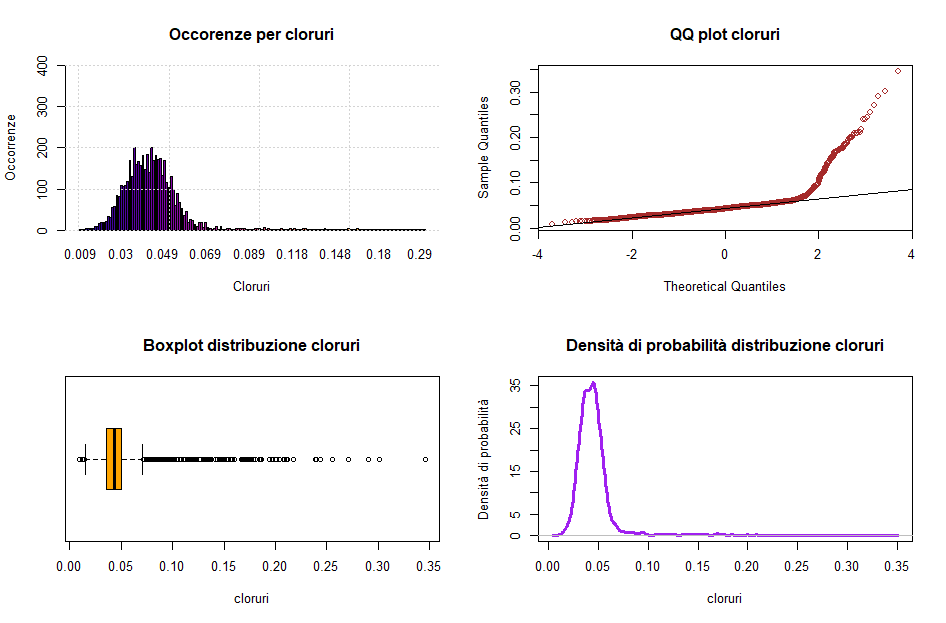
\includegraphics[width=1\textwidth]{immagini/clor.png}
    \caption{Plots per la descrizione della distribuzione della variabile di Cloruri}
\end{figure}
\FloatBarrier
Dall'insieme dei grafici relativi alla distribuzione dei cloruri è possibile concludere che la maggior parte dei valori seguano una distribuzione normale per bassi valori di cloruro. Invece si può notare come per alti valori cloruro, la distribuzione si discosta molto da una normale e appaiono quindi molti outliers.
\newpage
\subsubsection{Anidride Solforosa libera}
\begin{figure}[!htb]
    \centering
    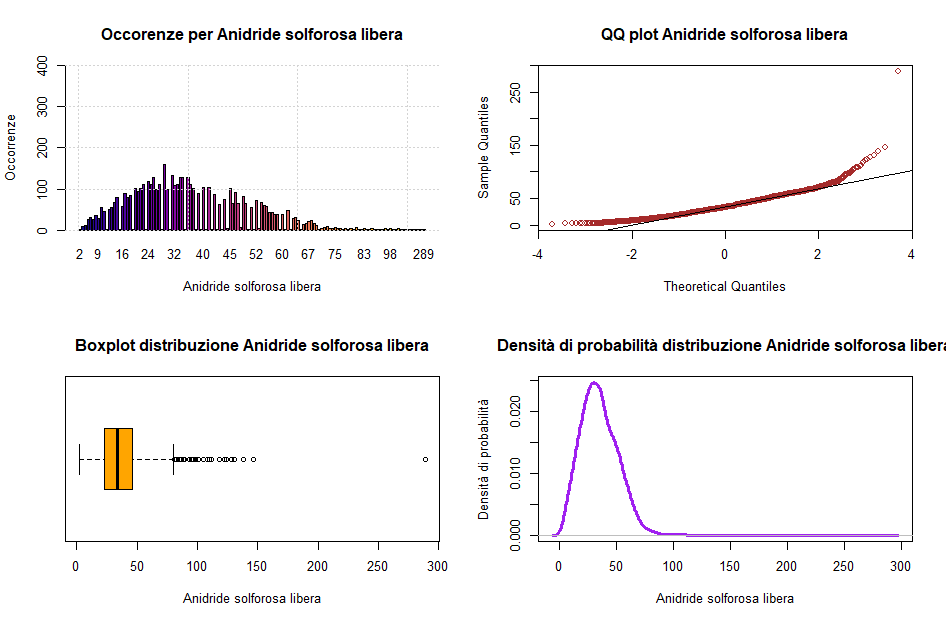
\includegraphics[width=1\textwidth]{immagini/anlib.png}
    \caption{Plots per la descrizione della distribuzione della variabile di Anidride Solforosa libera}
\end{figure}
\FloatBarrier
Dall'insieme dei grafici relativi alla distribuzione della variabile di Anidride Solforosa libera è possibile concludere che la maggior parte dei valori seguano una distribuzione normale, con l'eccezione di alcuni outlier per alti valori. Si può notare anche la presenza di un outlier in corrispondenza del valore di 300 mg/L. Molto al di sopra del limite consentito dalla legge europea (210 mg/l nei vini bianchi e rosati).
\newpage
\subsubsection{Anidride Solforosa totale}
\begin{figure}[!htb]
    \centering
    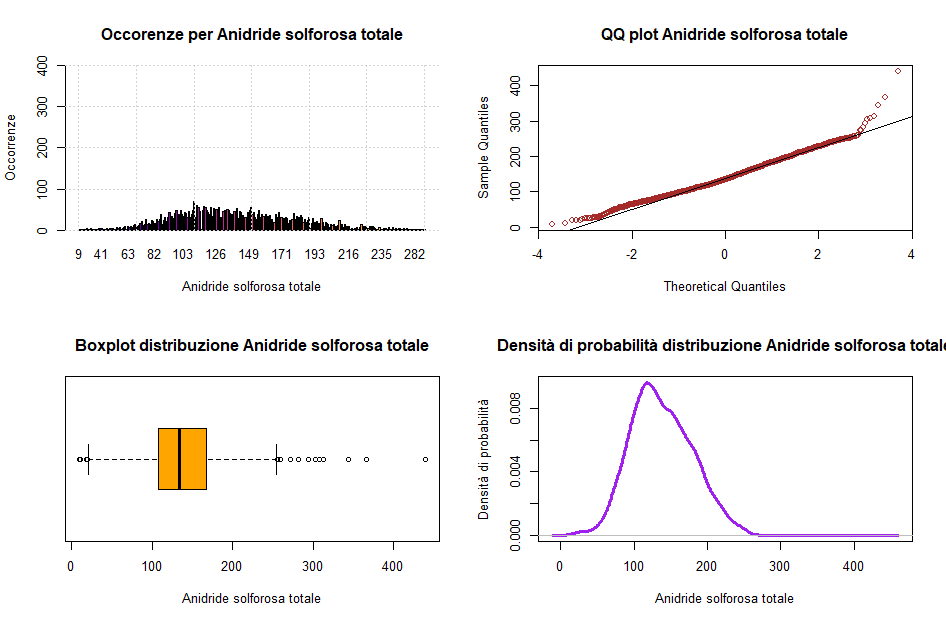
\includegraphics[width=1\textwidth]{immagini/antot.png}
    \caption{Plots per la descrizione della distribuzione della variabile di Anidride Solforosa totale}
\end{figure}
\FloatBarrier
Così come l'insieme dei grafici relativi alla distribuzione della variabile di Anidride Solforosa libera anche i grafici relativi alla distribuzione della variabile di Anidride Solforosa totale non si discostano molto da una distribuzione normale. Si può notare inoltre la minor presenza di outliers rispetto alla variabile precedente.
\newpage
\subsubsection{Densità}
\begin{figure}[!htb]
    \centering
    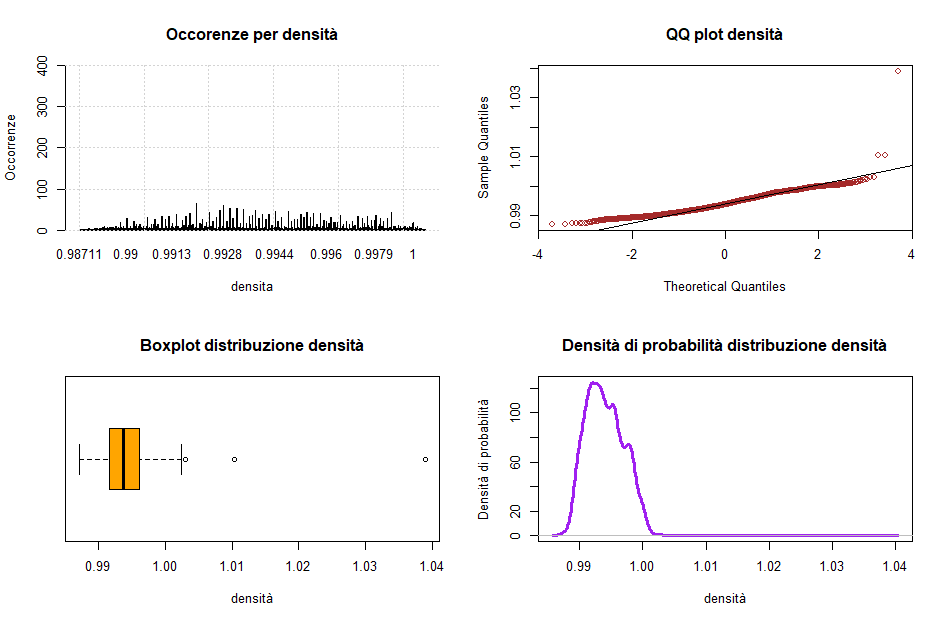
\includegraphics[width=1\textwidth]{immagini/den.png}
    \caption{Plots per la descrizione della distribuzione della variabile di Densità}
\end{figure}
\FloatBarrier
Dall'insieme dei grafici relativi alla distribuzione della variabile di Densità è possibile concludere che la quasi totalità di valori seguano una distribuzione normale, con l'eccezione di alcuni outlier per alti valori. In particolare si può notare un outlier in corrispondenza del valore di 1.04 di densità.
\newpage
\subsubsection{pH}
\begin{figure}[!htb]
    \centering
    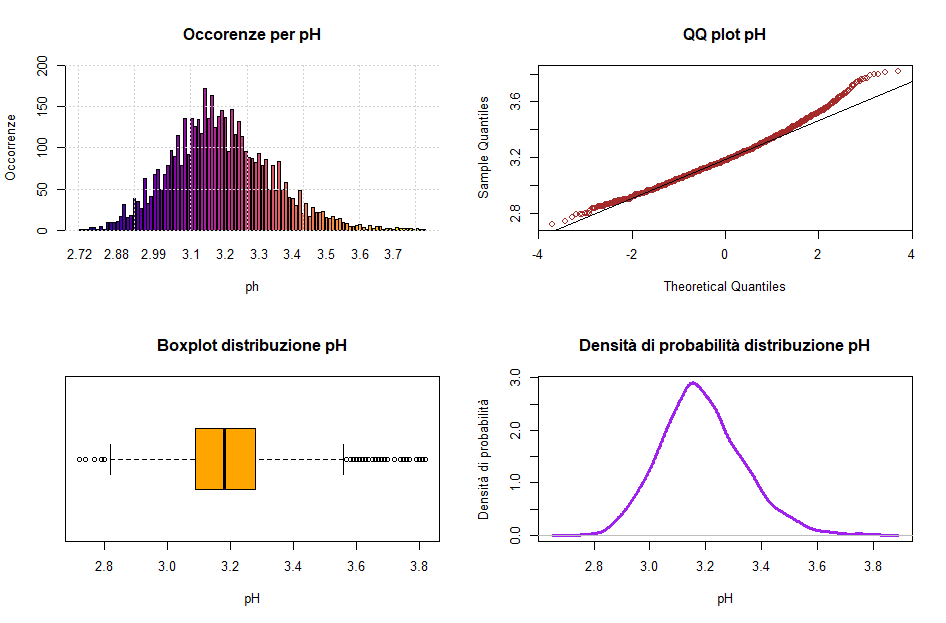
\includegraphics[width=1\textwidth]{immagini/ph.png}
    \caption{Plots per la descrizione della distribuzione della variabile di pH}
\end{figure}
\FloatBarrier
Così come l'insieme dei grafici relativi alla distribuzione della variabile di densità anche i grafici relativi alla distribuzione della variabile di pHnon si discostano per nulla da una distribuzione normale. Si può comunque notare la presenza di diversi outlier più concentrati su alti valori di pH
\newpage
\subsubsection{Solfati}
\begin{figure}[!htb]
    \centering
    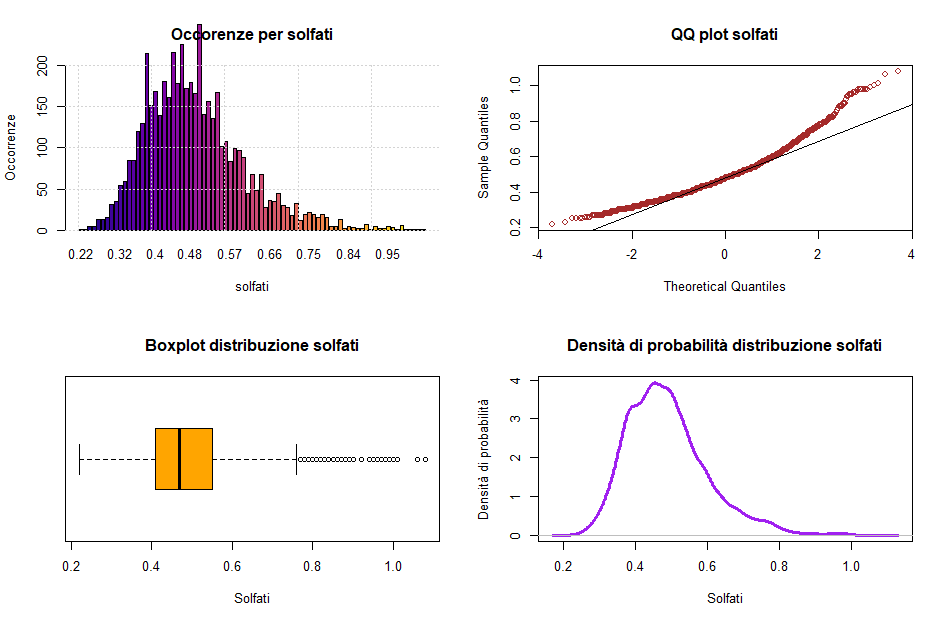
\includegraphics[width=1\textwidth]{immagini/solf.png}
    \caption{Plots per la descrizione della distribuzione della variabile di Solfati}
\end{figure}
\FloatBarrier
Anche la distribuzione della variabile relativa ai solfati non si discosta molto da una normale, anche se meno delle due variabili precedenti (ph e densità). Ci sono inoltre numerosi outliers per alti valori di solfati.
\newpage
\subsubsection{Percentuale di Alcol}
\begin{figure}[!htb]
    \centering
    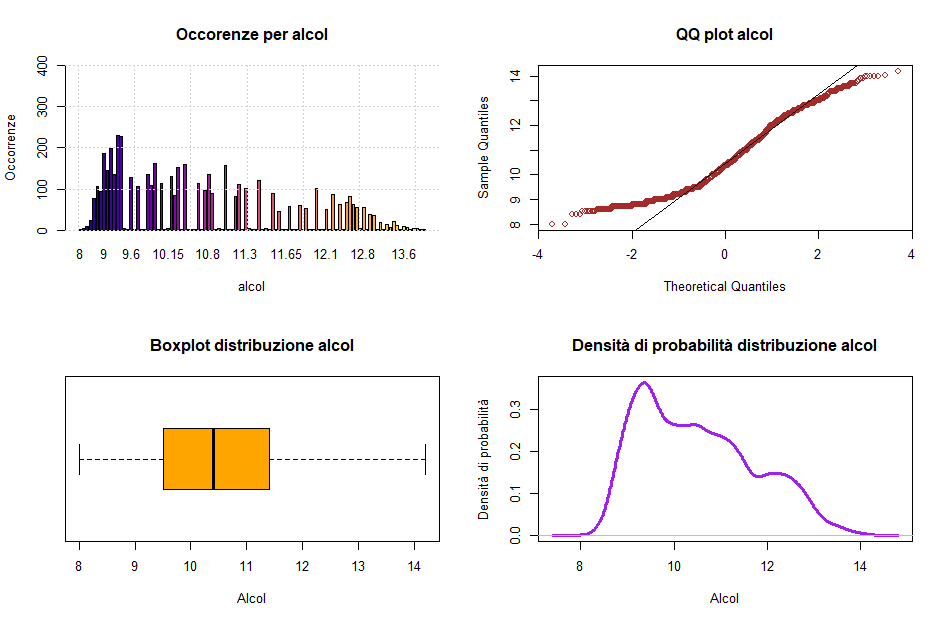
\includegraphics[width=1\textwidth]{immagini/alcol.png}
    \caption{Plots per la descrizione della distribuzione della variabile di Percentuale di Alcol}
\end{figure}
\FloatBarrier
La distribuzione della variabile di percentuale alcolica è discretamente regolare, infatti non presenta alcun outlier. Si può notare però dal Q-Q plot relativo come non sia distribuita propriamente secondo una normale.
\paragraph{Conclusione} Non presentando casi eccezionali di outliers o distribuzioni non regolari è possibile proseguire con l'analisi e i task di regressione e classificazione regolarmente senza intaccare l'integrità del dataset.
\newpage
\subsection{Correlazione tra variabili}
Utile ai fini dell'analisi è lo studio della matrice di correlazione tra le variabili del dataset per poter meglio comprendere da che parametri la qualità sia maggiormente "influenzata". Di seguito viene riportata una rappresentazione della matrice di correlaizone tra le variabili.
\begin{figure}[!htb]
    \centering
    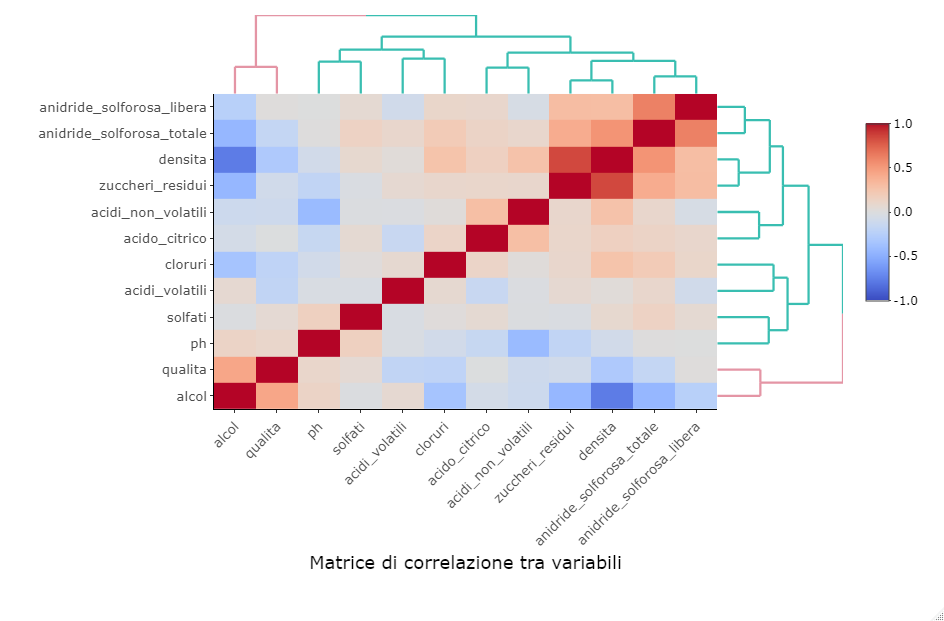
\includegraphics[width=1\textwidth]{immagini/cor.png}
    \caption{Matrice di correlazione tra le variabili}
\end{figure}
\FloatBarrier
Da una generica analisi della matrice di correlazione si può notare come la qualità del vino sia discretamente correlata (direttamente) con la percentuale alcolica e (inversamente) con la densità del vino. Ci si aspetta quindi che nei task di regressione e di classificazione vengano considerati con maggiore importanza questi due parametri.
\newpage
\section{Regressione e Classificazione}
\subsection{Organizzazione di training e test set}
Per l'applicazione di metodologie di predizione e classificazione e la loro valutazione il dataset è stato così suddiviso:
\begin{itemize}
    \item 85\% Training: 4163 Entries
    \item 15\% Test: 735 Entries
\end{itemize}
\subsection{Regressione}
\subsubsection{Regressione Lineare Multipla}
Il task prevede l'implementazione di modelli di regressione per la predizione della \textbf{qualità} dei vini in base alle loro proprietà chimiche. La formula iniziale che contiene tutte le variabili a disposizione prevede l'utilizzo della \textit{qualità} come variabile dipendente e la totalità delle altre variabili come variabili indipendenti.
\begin{figure}[!htb]
    \centering
    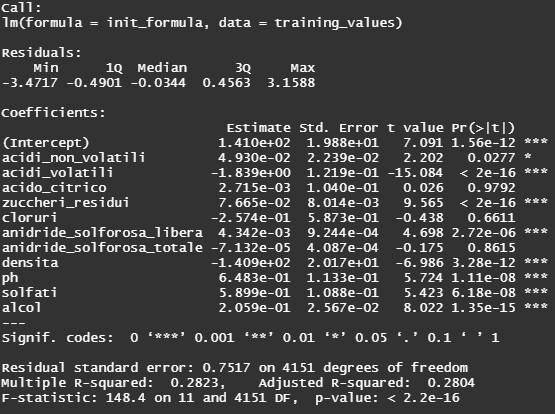
\includegraphics[width=0.6\textwidth]{immagini/init.png}
    \caption{Modello di regressione lineare multipla per la predizione della qualità del vino utilizzando tutte le variabili a disposizione}
\end{figure}
\FloatBarrier
Come si può notare ci sono delle variabili che non presentano una significatività sufficiente. Queste variabili vengono eliminate dal modello di regressione tramite l'utilizzo della tecnica di backward elimination. Un altro aspetto rilevante è il basso valore di adjusted R squared che denota una bassa efficacia del modello di predizione. Questo viene confermato anche dalla statistica relativa al Residual Standard Error, pari a 0.7517.
\begin{figure}[!htb]
    \centering
    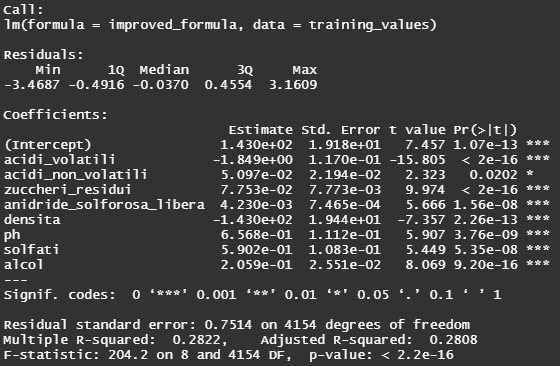
\includegraphics[width=0.6\textwidth]{immagini/impr.png}
    \caption{Modello di regressione lineare multipla per la predizione della qualità del vino utilizzando le variabili più significative}
\end{figure}
\FloatBarrier
Come si può notare il valore di adjusted R squared è aumentato di 0.0004, un incremento poco signifcativo per concludere di poter predire correttamente la qualità di un vino con un modello di regressione di questo tipo. Questo è confermato anche dalla stima del MAE (Mean Absoulte Error) che passa da un valore iniziale di 0.5935 a un valore di 0.5939.
\newpage
\subsubsection{Albero di regressione semplice}
Per implementare il task di regressione è possibile anche modellare un albero di decisione sulle variabili del dataset, ottenendo il modello seguente
\begin{figure}[!htb]
    \centering
    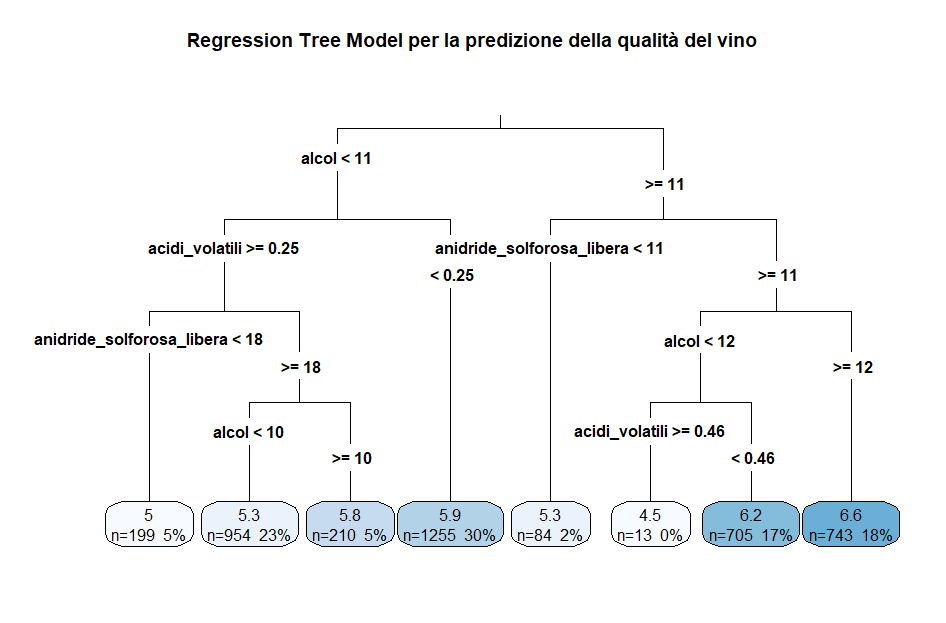
\includegraphics[width=1\textwidth]{immagini/regrtr.png}
    \caption{Modello di regressione ad albero per la predizione della qualità del vino utilizzando tutte le variabili}
\end{figure}
\FloatBarrier
Questo modello di regressione produce un MAE pari a 0.6103, un valore ancora peggiore rispetto ai modelli di regressione lineare multipla precedenti e quindi insufficiente.
\subsubsection{M5P}
M5P è una ristrutturazione dell'algoritmo M5 di Quinlan, dove viene combinato un albero decisionale convenzionale con la possibilità di aggiungere funzioni di regressione lineare nei nodi. Questo modello di regressione ha stimato i valori di qualità del test set ottenendo un MAE di 0.3887, nettamente inferiore ai modelli precedenti e accettabile per un modello di predizione.
\paragraph{Conclusione} L'unico modello accettabile per predire la qualità del vino in base alle sue caratteristiche chimiche è risultato essere l'M5P. Anche se non ottimale, risulta comunque essere un discreto strumento da utilizzare. Di seguito il sommario dei MAE dei vari modelli di regressione.
\begin{figure}[!htb]
    \centering
    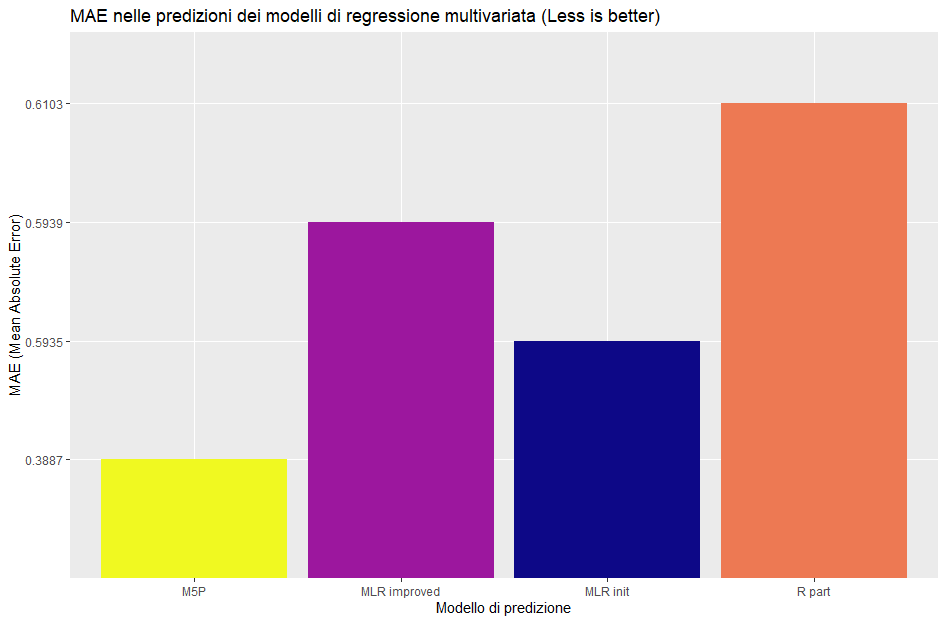
\includegraphics[width=1\textwidth]{immagini/mae.png}
    \caption{Sommario dei MAE dei modelli di regressione}
\end{figure}
\FloatBarrier
\newpage
\subsection{Classificazione}
\subsubsection{Introduzione}
Per effettuare una classificazione affidabile della qualità dei vini è stato deciso di suddividere il dataset utilizzando una feature aggiuntiva (gusto), che raggruppa la qualità dei vini in tre macrogruppi: di buon gusto (qualità $>$ 6), di normale gusto (qualità = 6) e di cattivo gusto (qualità $<$ 6). Di seguito il numero di occorrenze per gruppo:
\begin{figure}[!htb]
    \centering
    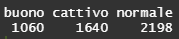
\includegraphics[width=0.4\textwidth]{immagini/gusto.png}
    \caption{Occorrenze di vino per gusto}
\end{figure}
\FloatBarrier
\newpage
\subsubsection{Albero di classificazione semplice}
Per una semplice classificazione della qualità del vino è possibile utilizzare ancora un modello decisionale ad albero. Di seguito la sua applicazione:
\begin{figure}[!htb]
    \centering
    \includegraphics[width=1\textwidth]{immagini/treecò.png}
    \caption{Albero di classificazione dei vini}
\end{figure}
Dopo la predizione della classificazione dei vini e il confronto con i dati reali è stata ottenuta la seguente matrice di confusione
\begin{figure}[!htb]
    \centering
    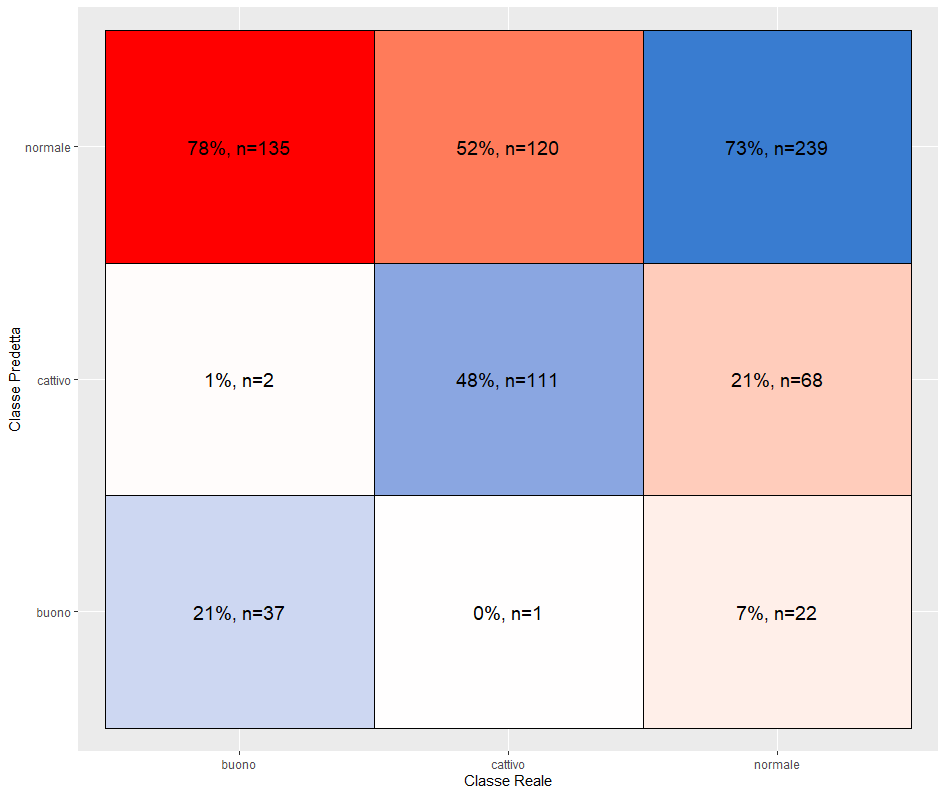
\includegraphics[width=1\textwidth]{immagini/simpleconf.png}
    \caption{Matrice di confusione per il modello di classificazione ad albero semplice}
\end{figure}
\FloatBarrier
La predizione tramite quello modello ha ottenuto un'accuracy pari al 52.65\%, un valore poco accettabile.
\newpage
\subsubsection{Random Forest}
Un altro metodo di classificazione implementabile è quello Random Forest. Partendo da un modello che fa uso di 100 alberi di decisione viene ottenuto il seguente risultato:
\begin{figure}[!htb]
    \centering
    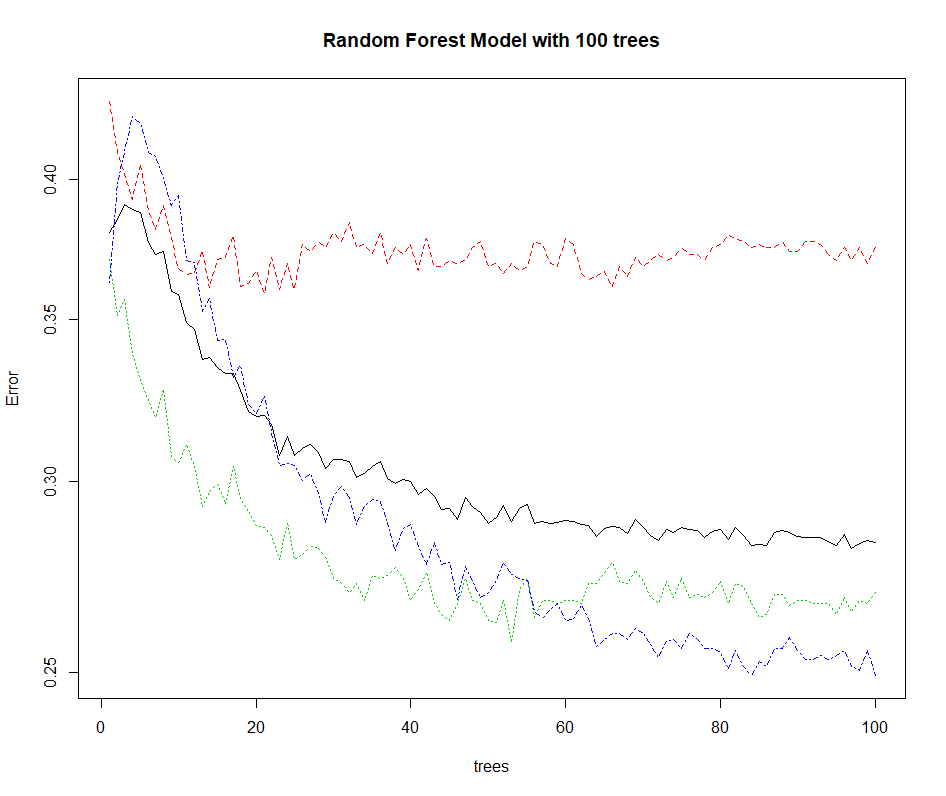
\includegraphics[width=1\textwidth]{immagini/100.png}
    \caption{Modello Random Forest con 100 alberi di decisione}
\end{figure}
\FloatBarrier
E la corrispondente matrice di confusione:
\begin{figure}[!htb]
    \centering
    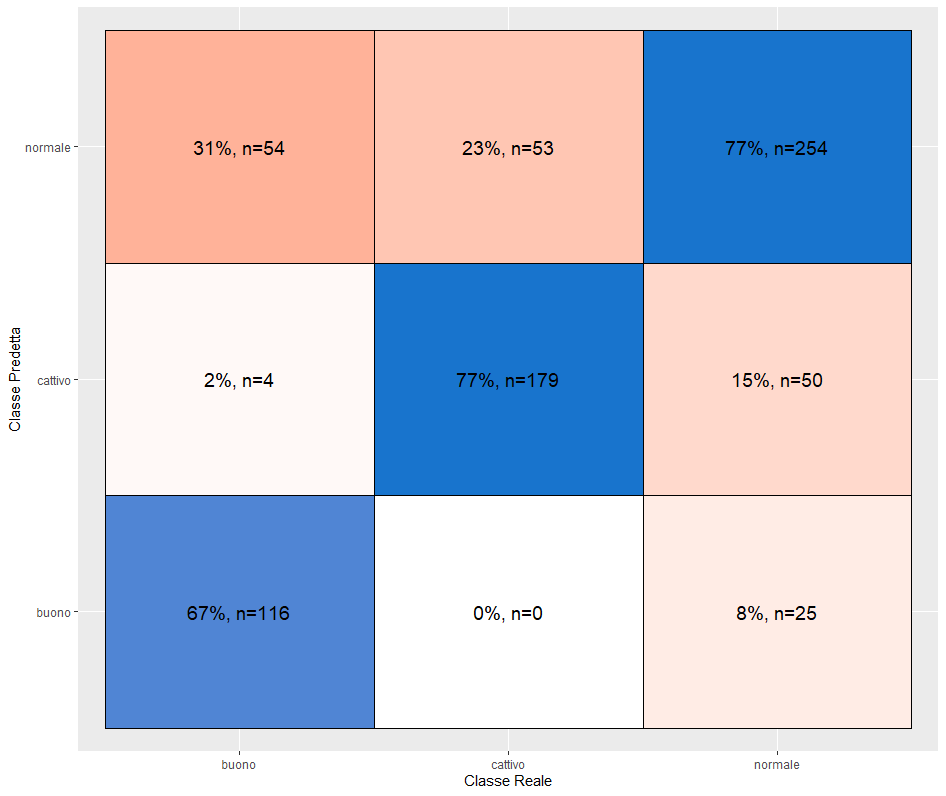
\includegraphics[width=1\textwidth]{immagini/conf100.png}
    \caption{Matrice di confusione random forest con 100 alberi}
\end{figure}
\FloatBarrier
La predizione Random Forest con 100 alberi di decisione ha prodotto un'accuracy del 74.69\% un valore più che accettabile e di gran lunga superiore rispetto a quello prodotto dall'utilizzo di un albero di decisione semplice. Aumentando il numero di alberi prodotti da Random Forest si raggiungono risultati pressoché simili. Di seguito le matrici di confusione associate:
\begin{figure}[!htb]
    \centering
    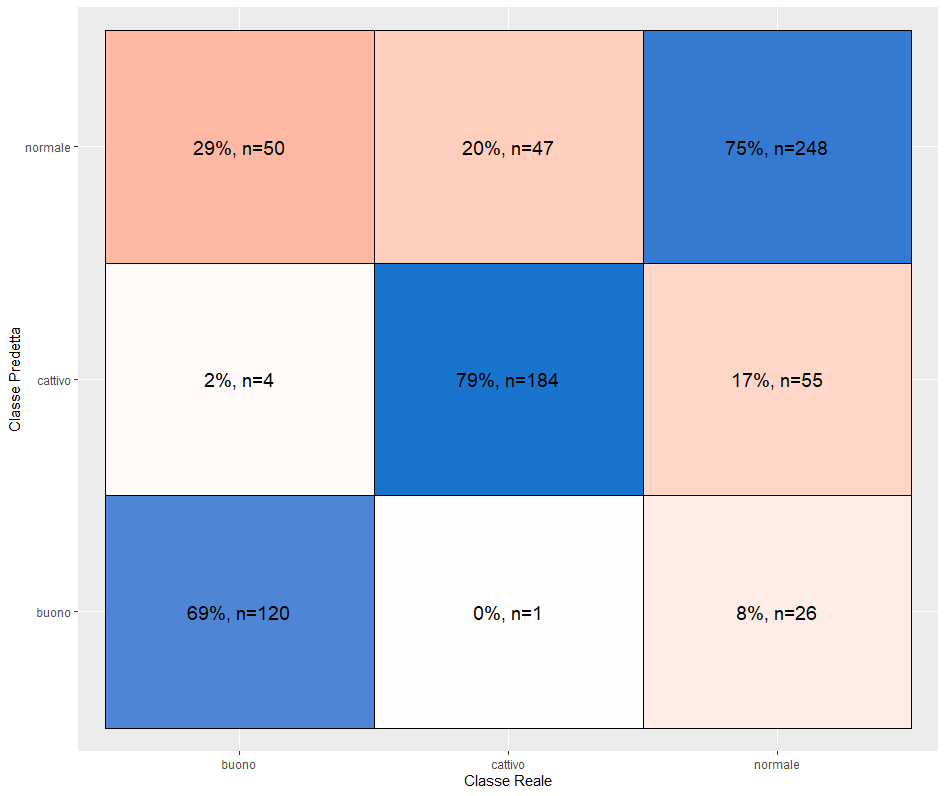
\includegraphics[width=1\textwidth]{immagini/conf200.png}
    \caption{Matrice di confusione random forest con 200 alberi}
\end{figure}
\FloatBarrier
Precisione: 75.1\%
\begin{figure}[!htb]
    \centering
    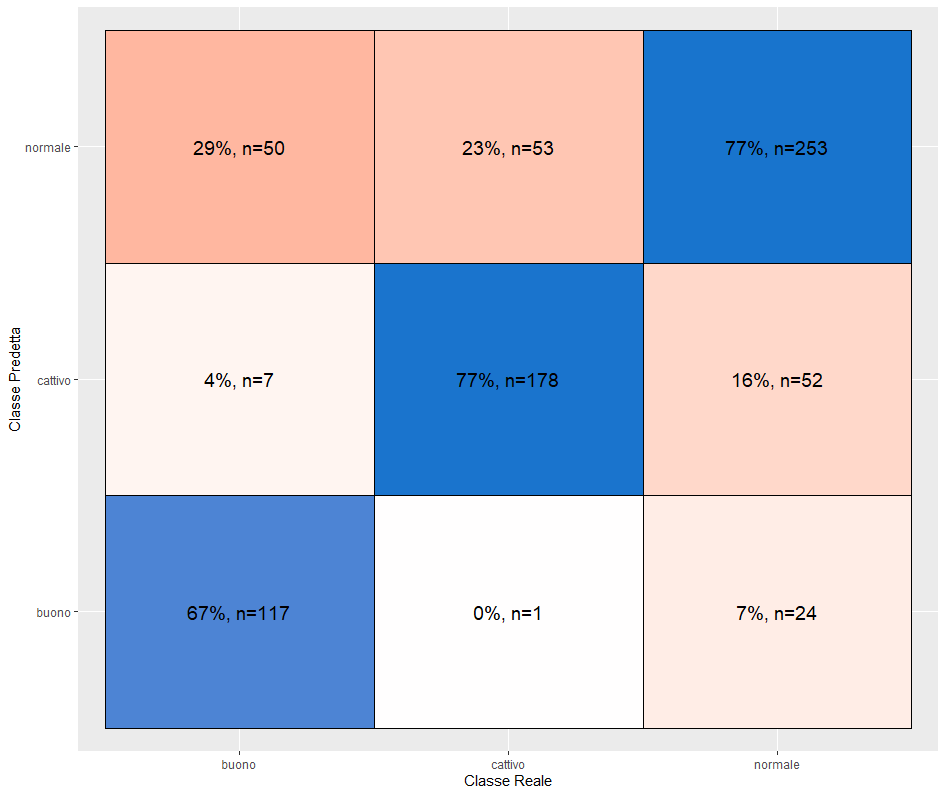
\includegraphics[width=1\textwidth]{immagini/300conf.png}
    \caption{Matrice di confusione random forest con 300 alberi}
\end{figure}
\FloatBarrier
Precisione: 74.56\%
\begin{figure}[!htb]
    \centering
    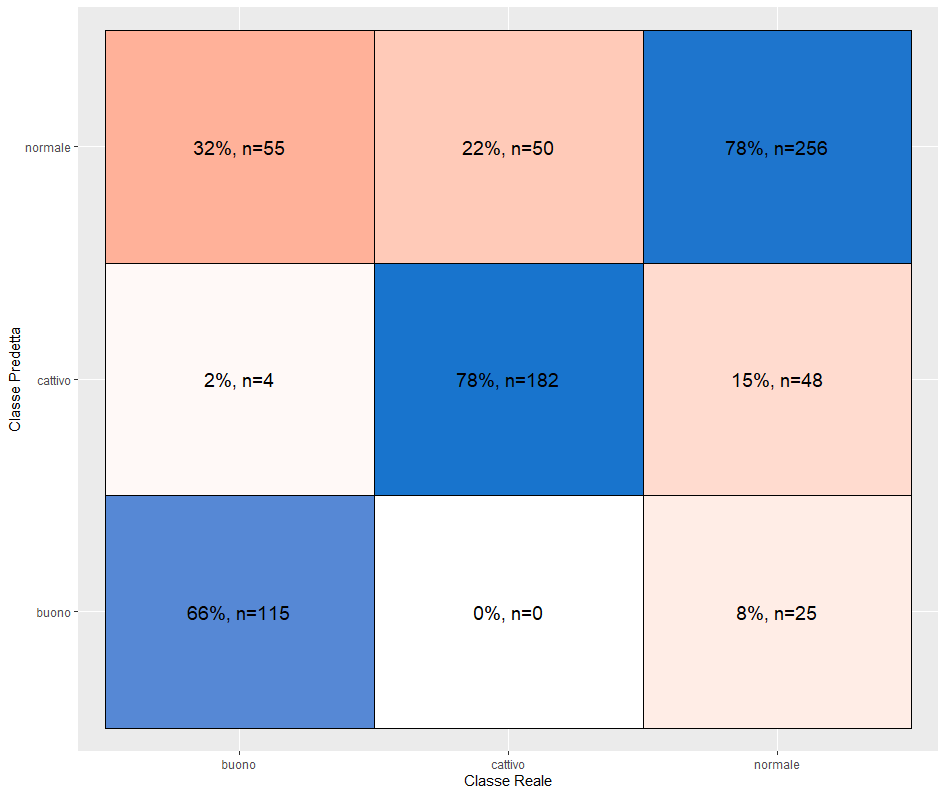
\includegraphics[width=1\textwidth]{immagini/conf400.png}
    \caption{Matrice di confusione random forest con 400 alberi}
\end{figure}
\FloatBarrier
Precisione: 75.24\%
\paragraph{Conclusioni} Dai modelli di classificazione presentati si evince che il migliore sia di gran lunga il random forest. Il numero di alberi utilizzati non influisce di molto sull'accuratezza dei risultati finali, quindi per avere migliori prestazioni è raccomandabile l'utilizzo del modello con 100 alberi. Di seguito il sommario dei risultati di accuratezza dei vari modelli:
\begin{figure}[!htb]
    \centering
    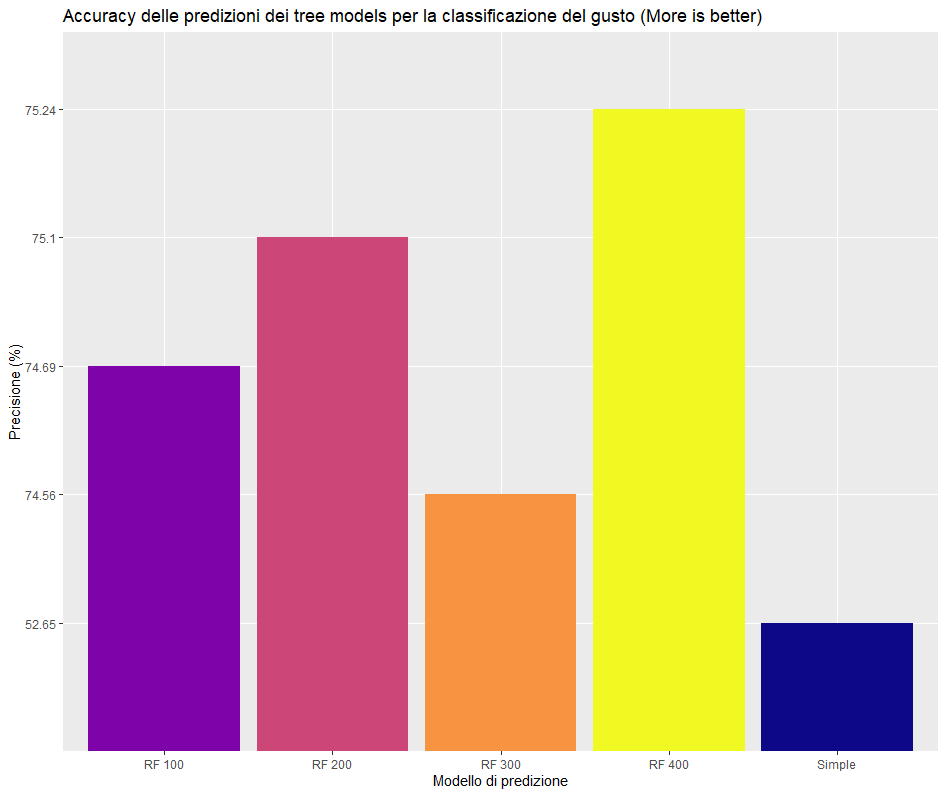
\includegraphics[width=1\textwidth]{immagini/acc.png}
    \caption{Accuratezza dei modelli di classificazione}
\end{figure}
\FloatBarrier

\section{Conclusioni}
Dall'analisi dei dati prodotti dai modelli di regressione è possibile concludere che le proprietà chimiche in analisi non sono ottimali per una corretta stima della qualità del vino. È stato possibile però, dopo aver raggruppato i vini in base alla qualità in 3 macro gruppi, effettuare una classificazione con discreti risultati. In particolare mediante l'implementazione di Random Forest è stato possibile raggiungere un'accuratezza del 75\%, questo denota come sia possibile stabilire il gusto di un vino particolarmente bene tra cattivo, normale e buono in base alle sue proprietà chimiche.
\end{document}